\documentclass[usenames,dvipsnames,tikz]{standalone}
\usepackage{xcolor}
\colorlet{tBlue}{RoyalBlue!35!Cerulean}
\colorlet{tRed}{Red}
\definecolor{tGreen}{HTML}{569909}
\definecolor{tOrange}{HTML}{FA7602} %tikz color
\usepackage{tikz}
\usepackage{standalone}
\begin{document}
	
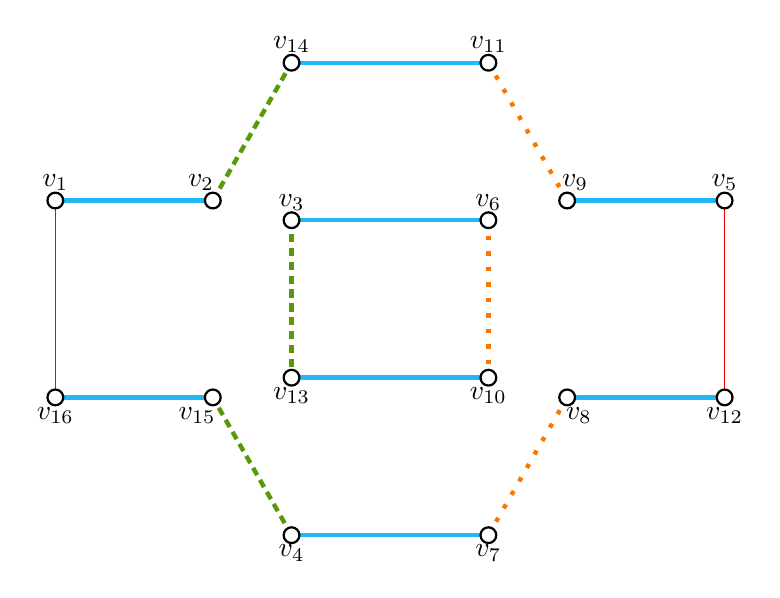
\begin{tikzpicture}
%\draw [help lines] (-1,-1) grid (15, 8);

%C1 - blue
\draw [ultra thick, tBlue] (0,1.75) -- (2,1.75);
\draw [ultra thick, tBlue] (0,4.25) -- (2,4.25); 


%C2 - blue
\draw [ultra thick, tBlue] (3,4) -- (5.5,4); 
\draw [ultra thick, tBlue] (3,6) -- (5.5,6);

%C3 - blue
\draw [ultra thick, tBlue] (3,0) -- (5.5,0);
\draw [ultra thick, tBlue] (3,2) -- (5.5,2);

%C4 - blue
\draw [ultra thick, tBlue] (6.5,1.75) -- (8.5,1.75);
\draw [ultra thick, tBlue] (6.5,4.25) -- (8.5,4.25);


%-------------------------------

%C1 - red
\draw [tRed] (0,1.75) -- (0,4.25); 
%\draw [tRed] (2,1.75) -- (2,4.25);


%C2 - red
%\draw [tRed] (3,4) -- (3,6);
%\draw [tRed] (5.5,4) -- (5.5,6);

%C3 - red
%\draw [tRed] (3,0) -- (3,2);
%\draw [tRed] (5.5,0) -- (5.5,2); 

%C4 - red
%\draw [tRed] (6.5,1.75) -- (6.5,4.25);
\draw [tRed] (8.5,1.75) -- (8.5,4.25); 

%C1 to C2 - green
\draw [ultra thick, densely dashed, tGreen] (2,4.25) -- (3,6); 
%C2 to C3 - green
\draw [ultra thick, densely dashed, tGreen] (3,4) -- (3,2);
%C3 to C1 - green
\draw [ultra thick, densely dashed, tGreen] (3,0) -- (2,1.75);  

%C2 to C3 - orange
\draw [ultra thick, loosely dotted, tOrange] (5.5,4) -- (5.5,2);
%C3 to C4 - orange
\draw [ultra thick, loosely dotted, tOrange] (5.5,0) -- (6.5,1.75);
%C4 to C2 - orange
\draw [ultra thick, loosely dotted, tOrange] (6.5,4.25) -- (5.5,6);   


%----------------------------

%C1 - vertices
\draw [fill=white, thick] (0,1.75) circle [radius = 0.1]; %v16
\draw [fill=white, thick] (2,1.75) circle [radius = 0.1]; %v15
\draw [fill=white, thick] (0,4.25) circle [radius = 0.1]; %v1
\draw [fill=white, thick] (2,4.25) circle [radius = 0.1]; %v2


%C2 - vertices
\draw [fill=white, thick] (3,4) circle [radius = 0.1]; %v3
\draw [fill=white, thick] (5.5,4) circle [radius = 0.1]; %v6
\draw [fill=white, thick] (3,6) circle [radius = 0.1]; %v14
\draw [fill=white, thick] (5.5,6) circle [radius = 0.1]; %v11

%C3 - vertices
\draw [fill=white, thick] (3,0) circle [radius = 0.1]; %v4
\draw [fill=white, thick] (5.5,0) circle [radius = 0.1]; %v7
\draw [fill=white, thick] (3,2) circle [radius = 0.1]; %v13
\draw [fill=white, thick] (5.5,2) circle [radius = 0.1]; %v10

%C4 - vertices
\draw [fill=white, thick] (6.5,1.75) circle [radius = 0.1]; %v8
\draw [fill=white, thick] (8.5,1.75) circle [radius = 0.1]; %v12
\draw [fill=white, thick] (6.5,4.25) circle [radius = 0.1]; %v9
\draw [fill=white, thick] (8.5,4.25) circle [radius = 0.1]; %v5


%C1 - labels
\node [below] at (0,1.75) {$v_{16}$};
\node [below] at (1.8,1.75) {$v_{15}$};
\node [above] at (0,4.25) {$v_1$};
\node [above] at (1.85,4.25) {$v_2$};


%C2 - labels
\node [above] at (3,4) {$v_3$};
\node [above] at (5.5,4) {$v_6$};
\node [above] at (3,6) {$v_{14}$};
\node [above] at (5.5,6) {$v_{11}$};

%C3 - labels
\node [below] at (3,0) {$v_4$};
\node [below] at (5.5,0) {$v_7$};
\node [below] at (3,2) {$v_{13}$};
\node [below] at (5.5,2) {$v_{10}$};


%C4 - labels
\node [below] at (6.65,1.75) {$v_8$};
\node [below] at (8.5,1.75) {$v_{12}$};
\node [above] at (6.6,4.25) {$v_9$};
\node [above] at (8.5,4.25) {$v_5$};

%Component labels
%\node at (1,3) {\Large{$C_1$}};
%\node at (4.25,5) {\Large{$C_2$}};
%\node at (4.25,1) {\Large{$C_3$}};
%\node at (7.5,3) {\Large{$C_4$}};


\end{tikzpicture}
	
\end{document}
